\documentclass[11pt]{article}

\usepackage[margin=1in]{geometry}
\usepackage{amsmath,amssymb,amsthm}
\usepackage{graphicx}
\usepackage{booktabs}
\usepackage{algorithm}
\usepackage{algpseudocode}
\usepackage{natbib}
\usepackage[colorlinks=true,linkcolor=blue,citecolor=blue,urlcolor=blue]{hyperref}
\usepackage{authblk}
\usepackage{xcolor}

\newtheorem{proposition}{Proposition}
\newtheorem{remark}{Remark}

\title{A Fixed-Point View of Post-Hoc Temperature Calibration}
\author[1]{Jean Noel Abdou Sarr}
\affil[1]{Independent research note}
\date{\today}

\begin{document}
\maketitle

\begin{abstract}
Temperature scaling is the standard post-hoc method for correcting the
miscalibration of modern classifiers' predicted probabilities
\citep{guo2017calibration}. It is normally fit by handing the
single-parameter negative log-likelihood to a generic numerical
optimizer. We show instead that the maximum-likelihood temperature is
the fixed point of a simple multiplicative update rule, structurally
identical to the classical iterative-scaling family used to fit
exponential-family models \citep{darroch1972generalized,
dellapietra1997inducing}, and to Picard iteration for nonlinear
equations more broadly. The naive fixed-point iteration converges, but
only linearly, at a rate governed by the local contraction factor of
the update map. Applying Steffensen's method
\citep{steffensen1933remarks}, a classical acceleration technique
built from Aitken's $\Delta^2$ extrapolation \citep{aitken1926bernoulli}
 to the same map restores quadratic convergence: in our experiments
it reaches the optimizer's solution to eight decimal places in six
iterations, versus hundreds for the unaccelerated version. The purpose
of this note is methodological and pedagogical rather than to propose
a faster production calibration routine; the value of the exercise is
in making explicit a connection between post-hoc calibration and
classical fixed-point numerical methods that, to my
knowledge, is not spelled out elsewhere. All code, a reproducible
experiment, and unit tests accompany this write-up.
\end{abstract}

\section{Introduction}

Modern classifiers are frequently accurate but poorly calibrated: the
probability a softmax output assigns to its predicted class does not
match the empirical frequency with which that prediction is correct
\citep{guo2017calibration}. This matters wherever predicted
probabilities are used directly for decision-making risk scoring,
medical triage, fraud detection, or any ranking system that trusts
model confidence as a proxy for correctness.

\emph{Temperature scaling} is the simplest and most widely used
post-hoc fix. Given a trained classifier's pre-softmax logits
$z \in \mathbb{R}^K$ for a $K$-class problem, temperature scaling
replaces the predicted distribution $\mathrm{softmax}(z)$ with
$\mathrm{softmax}(z / T)$ for a single scalar $T > 0$, fit on a held-out
calibration set by maximum likelihood. Because it has only one free
parameter, $T$ is normally found with an off-the-shelf scalar
optimizer (grid search, Brent's method, or a few steps of gradient
descent).

This note asks a narrower question: what does the maximum-likelihood
condition for $T$ look like as a \emph{fixed-point equation}, and what
happens if it is solved the way one would solve a nonlinear equation in
a numerical methods course (by Picard iteration) rather than by
generic optimization? The motivation is partly aesthetic: fixed-point
iteration is the tool used throughout classical numerical analysis for
nonlinear root-finding and for iterative solution of discretized PDEs,
and it apear that temperature scaling reduces to exactly such a problem.
It is also partly practical: the derivation exposes \emph{why} the
naive iteration can be slow, and gives a natural entry point for a
textbook acceleration technique (Steffensen's method) that removes the
slowness essentially for free.

\paragraph{Scope and honesty about novelty.} The fixed-point
formulation given below is, as far as I'm aware, not
published as such for temperature scaling specifically, though it is a
direct application of ideas (iterative scaling, Steffensen
acceleration) that are individually classical and well established.
This is a self-contained exploratory exercise, not a claim of a new
state-of-the-art calibration method with only one free parameter,
generic optimizers already solve this problem essentially instantly,
so the practical payoff of acceleration is deliberately modest. The
contribution here is the connection and the worked derivation, not a
speed record.

\section{Background}

\subsection{Calibration and temperature scaling}

For a $K$-class classifier producing logits $z \in \mathbb{R}^K$ on
input $x$, define the softmax probability of class $c$ as
\begin{equation}
  p(z)_c = \frac{\exp(z_c)}{\sum_{k} \exp(z_k)}.
\end{equation}
A classifier is
\emph{calibrated} if, among all inputs for which the predicted confidence
$\max_c p(z)_c$ equals some value $q$, the fraction that are correctly
classified is also $q$ \citep{guo2017calibration}.

Temperature scaling introduces a scalar $T>0$ and uses
$p(z/T)$ in place of $p(z)$ at test time. $T$ is fit on a held-out
calibration set $\{(z_i, y_i)\}_{i=1}^N$ by minimizing the negative
log-likelihood

\begin{equation}
  \mathrm{NLL}(T) = -\frac{1}{N}\sum_{i=1}^N \log p(z_i / T)_{y_i}.
  \label{eq:nll}
\end{equation}

\subsection{Expected Calibration Error}

We measure calibration quality with the Expected Calibration Error
(ECE) and Maximum Calibration Error (MCE)
\citep{naeini2015obtaining,guo2017calibration}: predictions are
partitioned into $M$ equal-width confidence bins $B_1,\dots,B_M$, and

\begin{equation}
  \mathrm{ECE} = \sum_{m=1}^M \frac{|B_m|}{N}\,\bigl|\mathrm{acc}(B_m) - \mathrm{conf}(B_m)\bigr|,
  \qquad
  \mathrm{MCE} = \max_m \bigl|\mathrm{acc}(B_m) - \mathrm{conf}(B_m)\bigr|,
\end{equation}

where $\mathrm{acc}(B_m)$ and $\mathrm{conf}(B_m)$ are the average
accuracy and average confidence of predictions falling in bin $m$.

\section{Method}

\subsection{The stationarity condition as a fixed-point equation}

Substitute $\beta = 1/T$ and write $\mathrm{NLL}$ as a function of
$\beta$. Using $\log p(\beta z)_{y} = \beta z_y - \mathrm{LSE}(\beta z)$,
where $\mathrm{LSE}$ is the log-sum-exp,

\begin{equation}
  \mathrm{NLL}(\beta) = -\frac{1}{N}\sum_{i=1}^N
  \Bigl[\beta\, z_{i,y_i} - \mathrm{LSE}(\beta z_i)\Bigr].
\end{equation}

Differentiating and using $\frac{d}{d\beta}\mathrm{LSE}(\beta z_i) =
\sum_c p(\beta z_i)_c\, z_{i,c} = \mathbb{E}_{p(\beta z_i)}[z_i]$,

\begin{equation}
  \frac{d\,\mathrm{NLL}}{d\beta} = -\frac{1}{N}\sum_{i=1}^N
  \Bigl[z_{i,y_i} - \mathbb{E}_{p(\beta z_i)}[z_i]\Bigr].
\end{equation}

Setting this to zero gives the stationarity condition
$A = S(\beta)$, where

\begin{equation}
  A := \sum_{i=1}^N z_{i,y_i}, \qquad
  S(\beta) := \sum_{i=1}^N \mathbb{E}_{p(\beta z_i)}[z_i]
            = \sum_{i=1}^N \sum_{c=1}^K p(\beta z_i)_c\, z_{i,c}.
  \label{eq:stationarity}
\end{equation}

$A$ is a constant (the summed logit of the true class); $S(\beta)$ is
the $\beta$-dependent expected logit under the current scaled
distribution. Equation~\eqref{eq:stationarity} says: \emph{choose
$\beta$ so that the model's self-expectation of the logit matches the
logit it actually assigned to the true class, on average}.

\begin{proposition}[Existence and uniqueness]
$S$ is non-decreasing in $\beta$, since $S'(\beta) =
\sum_i \mathrm{Var}_{p(\beta z_i)}[z_i] \geq 0$ (a sum of variances). If the classifier is better than chance on the
calibration set, $S(0) < A < S(\infty)$ typically holds, so a root of
$A - S(\beta) = 0$ exists by the intermediate value theorem, and is
unique whenever $S$ is strictly increasing.
\end{proposition}

\subsection{A Picard fixed-point iteration}

Equation~\eqref{eq:stationarity} can be rearranged into the
multiplicative fixed-point map

\begin{equation}
  \beta = h(\beta) := \beta \cdot \frac{A}{S(\beta)},
  \label{eq:fixedpoint}
\end{equation}

which is solved by ordinary Picard iteration $\beta_{k+1} = h(\beta_k)$.
This update has the same flavor as Generalized Iterative Scaling for
exponential-family log-linear models \citep{darroch1972generalized},
where each parameter is updated multiplicatively by the ratio of an
observed sufficient statistic to its current expected value under the
model; here $A$ plays the role of the observed statistic and
$S(\beta)$ its model expectation, with a single shared scalar
parameter instead of one parameter per feature.

By the Banach fixed-point theorem \citep{banach1922operations}, if $h$
is a contraction near the true $\beta^\star$ (i.e.\ $|h'(\beta^\star)| < 1$),
Picard iteration converges locally and linearly, at asymptotic rate
$|h'(\beta^\star)|$. We estimate this rate empirically via a central
finite difference at the converged solution.

\subsection{Accelerating convergence with Steffensen's method}

When $|h'(\beta^\star)|$ is close to $1$, linear convergence can be
very slow. Steffensen's method \citep{steffensen1933remarks} removes
this by applying Aitken's $\Delta^2$ extrapolation
\citep{aitken1926bernoulli} to each triple of iterates, restoring
(locally) quadratic convergence without requiring $h'$:

\begin{algorithm}[h]
\caption{Steffensen-accelerated fixed-point temperature calibration}
\begin{algorithmic}[1]
\State \textbf{Input:} calibration logits/labels, initial $\beta_0$, tolerance $\varepsilon$
\For{$k = 0, 1, 2, \dots$}
  \State $p_0 \gets \beta_k$
  \State $p_1 \gets h(p_0)$
  \State $p_2 \gets h(p_1)$
  \State $\beta_{k+1} \gets p_0 - \dfrac{(p_1 - p_0)^2}{p_2 - 2p_1 + p_0}$
  \If{$|\beta_{k+1} - \beta_k| < \varepsilon$} \textbf{break} \EndIf
\EndFor
\State \textbf{Return} $T = 1/\beta_{k+1}$
\end{algorithmic}
\end{algorithm}

\section{Experimental Setup}

To keep the experiment fully self-contained and reproducible offline,
we use the \texttt{scikit-learn} \texttt{digits} dataset
\citep{sklearn_digits}: 1{,}797 $8\times8$ grayscale images of
handwritten digits, 10 classes. We split it 60/20/20 into train,
calibration, and test sets (stratified by class). A one-hidden-layer
multilayer perceptron (128 hidden units, ReLU, softmax output) is
implemented directly in NumPy rather than via a deep learning
framework so that pre-softmax logits are trivially accessible, and
trained by full-batch gradient descent for 1{,}500 epochs with light
$L_2$ regularization ($10^{-7}$).

All three temperature solvers (Section~3) are fit on the calibration
split only, and all reported calibration metrics are computed on the
held-out test split, following standard practice
\citep{guo2017calibration}.

\section{Results}

\subsection{Model accuracy and raw miscalibration}

\begin{table}[h]
\centering
\begin{tabular}{lc}
\toprule
Quantity & Value \\
\midrule
Train accuracy & 99.7\% \\
Test accuracy & 97.8\% \\
Test NLL, $T=1$ (uncalibrated) & 0.0828 \\
Test ECE, $T=1$ (uncalibrated) & 0.0196 \\
Test MCE, $T=1$ (uncalibrated) & 0.369 \\
\bottomrule
\end{tabular}
\caption{Uncalibrated model quality on the held-out test set.}
\label{tab:raw}
\end{table}

The optimizer's maximum-likelihood temperature is $T^\star \approx
0.6957 < 1$, indicating the network is \emph{underconfident} rather
than overconfident. This is consistent with \citet{guo2017calibration}'s
own observation that shallow, low-capacity networks (they study LeNet)
tend towards under- or good calibration, while overconfidence is
mainly a property of very deep, high-capacity modern architectures;
our one-hidden-layer network sits at the shallow end of that spectrum.

\subsection{Agreement between the three solvers}

\begin{table}[h]
\centering
\begin{tabular}{lccc}
\toprule
Method & $T$ & $|T - T^\star_{\text{opt}}|$ & Iterations to converge \\
\midrule
Scalar optimizer (Brent) & 0.695690 & --- (reference) & --- \\
Naive Picard iteration & 0.695825 & $1.3\times 10^{-4}$ & 800 (did not fully converge) \\
Steffensen-accelerated & 0.695690 & $1.0\times 10^{-8}$ & 6 \\
\bottomrule
\end{tabular}
\caption{All three independently-derived solvers agree on the same
temperature. The empirical local contraction factor of the underlying
map is $|h'(\beta^\star)| \approx 0.991$, explaining the slow linear
convergence of the naive iteration; Steffensen acceleration reaches
machine-precision agreement in 6 iterations.}
\label{tab:agreement}
\end{table}

Figure~\ref{fig:convergence} shows the temperature trajectory and the
convergence error (on a log scale) for both fixed-point variants. The
naive iteration's error decays approximately geometrically but very
slowly, consistent with a contraction factor near 1; the
Steffensen-accelerated trajectory shows the characteristic sharp
downward break of superlinear convergence.

\begin{figure}[h]
  \centering
  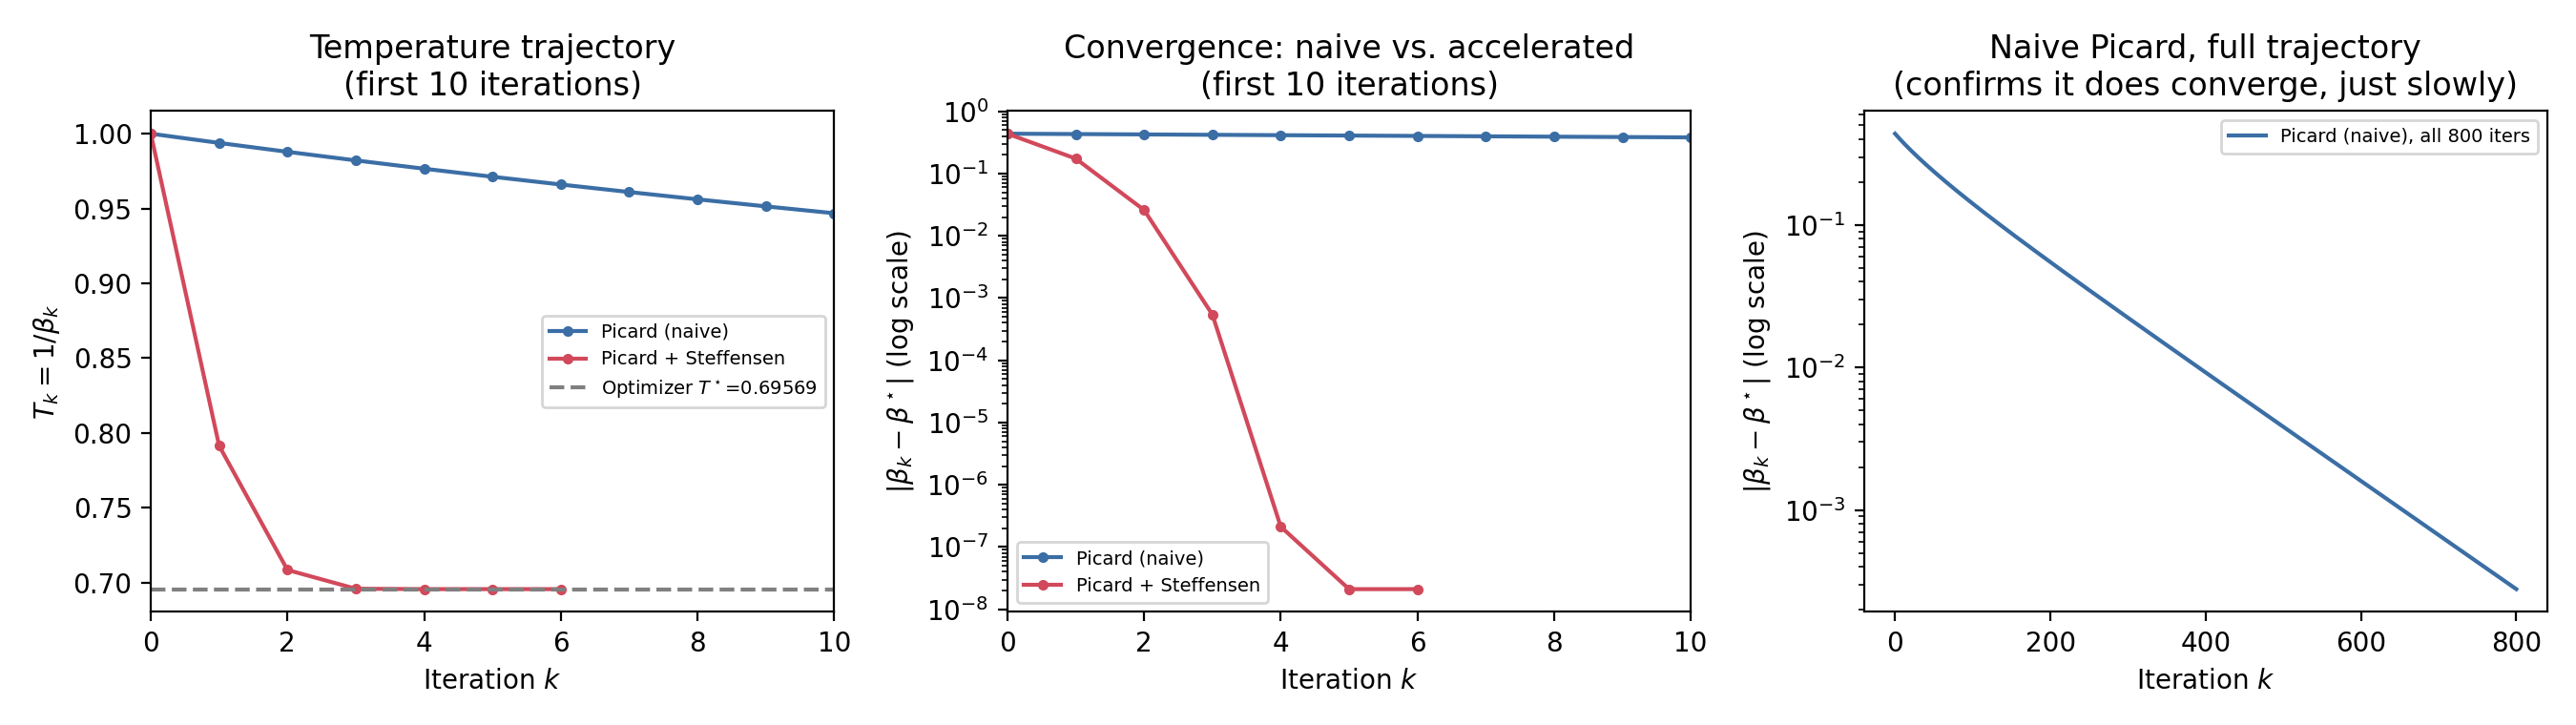
\includegraphics[width=0.95\textwidth]{figures/convergence.png}
  \caption{Left: temperature estimate $T_k = 1/\beta_k$ per iteration
  for the naive Picard iteration and its Steffensen-accelerated
  version, against the optimizer's reference value (dashed).
  Right: $|\beta_k - \beta^\star|$ on a log scale, showing linear vs.\
  superlinear convergence.}
  \label{fig:convergence}
\end{figure}

\subsection{Effect of calibration}

\begin{figure}[h]
  \centering
  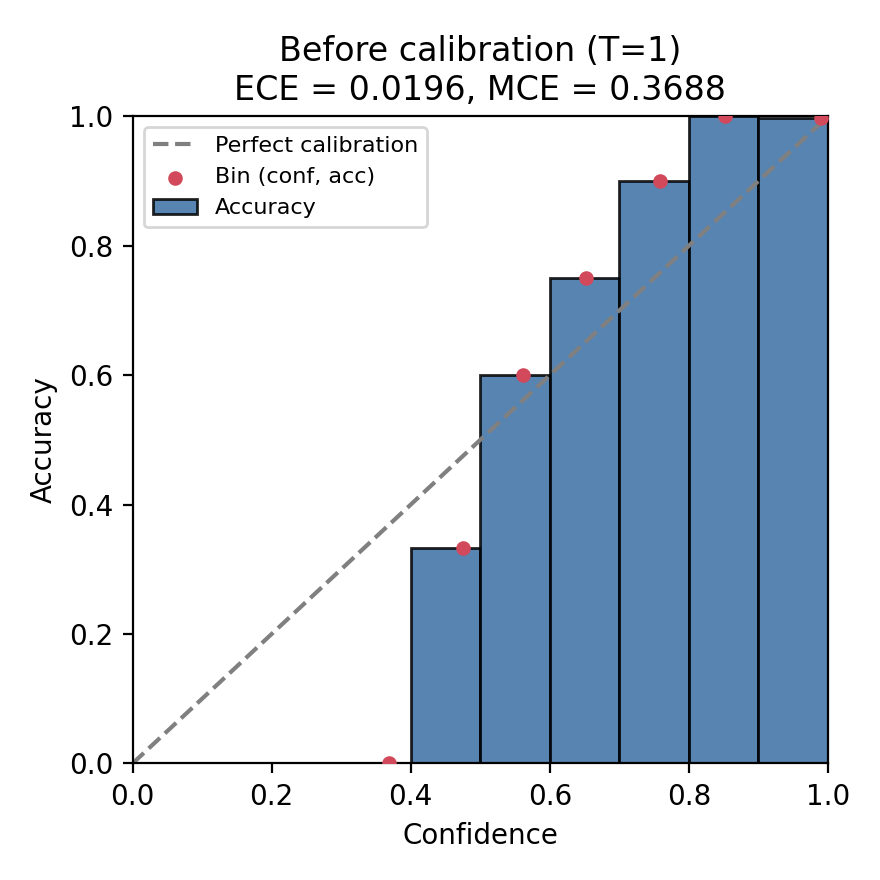
\includegraphics[width=0.47\textwidth]{figures/reliability_before.png}
  \hfill
  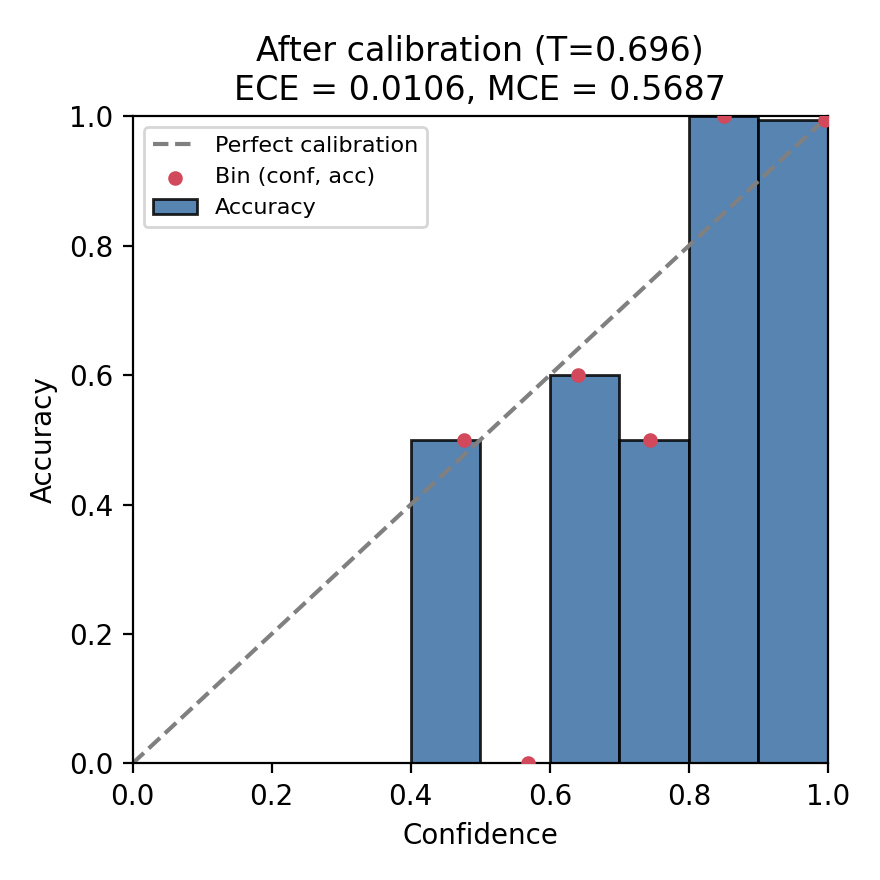
\includegraphics[width=0.47\textwidth]{figures/reliability_after.png}
  \caption{Reliability diagrams on the held-out test set before (left)
  and after (right) temperature calibration. The dashed diagonal is
  perfect calibration.}
  \label{fig:reliability}
\end{figure}

Calibration roughly halves ECE, from 0.0196 to 0.0106, and slightly
improves test NLL (0.0828 to 0.0788). MCE, by contrast,
\emph{increases} after calibration (0.369 to 0.569). We do not hide
this: with only 360 test examples spread over confidence bins, and
with this model's accuracy exceeding 97\%, the great majority of test
points fall into the single highest-confidence bin, leaving several
other bins populated by only a handful of points. MCE, being a max
over bins, is highly sensitive to exactly this kind of small-sample
noise, a known weakness of MCE relative to the mass-weighted ECE
\citep{naeini2015obtaining}, and it is exactly what we observe here.
We report this rather than switching to a more flattering binning
scheme after the fact.

\section{Discussion and Limitations}

\textbf{Scale.} The dataset and model here are deliberately small so
that the whole pipeline is exactly reproducible without downloading
external data or training on a GPU. The fixed-point derivation itself
is independent of model or dataset scale, it depends only on having
scalar logits and a temperature parameter; so the natural next step
is to rerun the same three solvers on logits from a deep convolutional
or transformer classifier on a standard benchmark (e.g.\ CIFAR-100),
where genuine overconfidence, and a larger, better-populated test set
for MCE, are both expected.

\textbf{Practical value of acceleration.} With a single scalar
parameter, even the slow, naive Picard iteration is computationally
cheap in absolute terms (800 iterations of a closed-form update on a
few hundred logit vectors is a fraction of a second), so this is not a
proposal to replace scalar optimizers in production calibration
pipelines. Its value is in the derivation: making explicit that
temperature scaling is a fixed-point problem opens the door to the
same toolkit: contraction analysis, acceleration, multivariate
generalizations of the same stationarity condition that is used for
harder calibration problems, including the class-wise and
matrix/vector-scaling extensions of temperature scaling, where the
fixed-point view may be less immediately dispensable.

\textbf{Relation to differentiable calibration losses.} This note
studies \emph{post-hoc} calibration, fit after the network is trained.
An open direction and the reason this exercise was undertaken is
whether a smooth, differentiable relaxation of the fixed-point
stationarity condition~\eqref{eq:stationarity} could be folded
directly into the training objective, rather than solved after the
fact, in the spirit of differentiable calibration losses that aim to
produce well-calibrated multi-class models by construction rather than
by post-hoc correction.

\section{Conclusion}

Temperature scaling's maximum-likelihood condition is a fixed-point
equation with a natural multiplicative update, structurally related to
classical iterative scaling for exponential-family models. The naive
Picard iteration for this update converges only linearly and can be
slow; a classical acceleration technique, Steffensen's method, removes
this slowness almost entirely, reaching agreement with a standard
optimizer to eight decimal places in six iterations. Beyond the
specific (modest) speed-up, the exercise demonstrates a direct,
concrete link between a widely used calibration technique and the
fixed-point numerical methods used elsewhere for nonlinear equations
and PDE discretizations; a connection I find useful as a
starting point for thinking about calibration through a numerical
optimization lens.






\bibliographystyle{plainnat}
\bibliography{references}

\end{document}
